%!TEX encoding = UTF-8 Unicode
\section{Related Work}
\label{sec:RelatedWork}
% Show what you read Start by presenting the structure of component. Show each
% item in a different section. Which works are known as relevant in this area
% Each section should end with a comparative evaluation. End each chapter with a
% synthesis, a table about various solutions, which features are interesting,
% which we want. Finnish sections with a work summary on a single sentence.

The solution proposed in this document leverages knowledge obtained from studying several concepts and systems from the current state-of-the-art. In this section, an overview of those concepts and systems will be given, stating for each of them their advantages and disadvantages. This section is structured as follows. Section \ref{sec:Computingparadigms} presents different methods to push intelligence and computing power closer to the source of the data and why this work adopted fog computing for this purpose. Finally, Section \ref{sec:fog_architecture} xxx, and \ref{sec:Migration} xxx. \ref{sec:Toolkits} xxx.

%!TEX encoding = UTF-8 Unicode
\subsection{Related Computing Paradigms}
\label{sec:Computingparadigms}
In what concerns fog computing standardization, there is a lack of unanimity. As aforementioned, fog has been variously termed as cloudlets, edge computing, etc. Different research teams are proposing many independent definitions of fog (and fog-related computing paradigms). As there is a research gap in the definitions and standards for fog computing, this work follows the definitions that Ashkan Yousefpour et al. \cite{yousefpour2018all} present. Below, are described some paradigms that were raised in order to bring cloud closer to the end devices, as well as their pros and cons. As a conclusion, we show why fog computing is the natural platform for IoT.

\subsubsection{Mobile Computing}\label{subsec:MC}
Mobile/Nomadic Computing (MC) is characterized by the processing being performed by mobile devices (e.g., laptops, tablets, or mobile phones). It is necessary to overcome the inherent limitations of environments where connectivity is sparse or intermittent and where there is low computing power. As this model only uses mobile devices to provide services to clients, there is no need for extra hardware. They already have communication modules such as Bluetooth, WiFi, ZigBee, etc. As already mentioned, mobile devices have evolved in recent years. However, their resources are more restricted, compared to fog and cloud. This computing paradigm has the advantage of being characterized by a distributed architecture. The disadvantages of MC are mainly due to their hardware nature (i.e. low resources, balancing between autonomy and the dependency of other mobile devices; characteristic that prevails in all distributed architectures) and the need for mobile clients to efficiently adapt to changing environments \cite{satyanarayanan1996fundamental}. MC alone may not be able to meet the requirements of some applications. On the one hand, it is limited due to autonomy constraints and, on the order hand by low computational and storage capacity. This restricts the applications where this paradigm is feasible. For instance, it is unsuitable for applications that require low-latency and which, at the same time, generate large amounts of data that needs to be stored or processed. Nonetheless, MC can use both fog and cloud computing to enhance its capacities, not being restricted to a local network, expanding the scope of mobile computing and the number of applications where it can be used.

\subsubsection{Mobile Cloud Computing}
Cloud and fog computing, as mentioned in Section \ref{subsec:MC}, are key elements for validate the importance of MC. This interaction between them results in a new paradigm, called mobile cloud computing (MCC). MCC, differs from MC in the sense that mobile applications can be partitioned at runtime, so that computationally intensive components of the application can be handled through adaptive offloading \cite{shiraz2013review}, from mobile devices to the cloud. This characteristic increases the autonomy of mobile devices (i.e battery lifetime), as both the data storage and data processing may occur outside of them. Also, it enables a much broader range of mobile subscribers, rather than the previous laptops, tablets, or mobile phones. Unlike the resource-constrained MC, MCC has high availability of computing resources, scaling the type of applications where it is possible to use (e.g., augmented reality applications). Unlike MC, MCC relies on cloud-based services, where its access is done through the network core by WAN connectivity, which means that applications running on these platforms require connection to the Internet all the time. On the one hand, both MCC and MC suffer from the intrinsic characteristics of mobility, such as frequent variations of network conditions (intensified under rapid mobility patterns), and, on the other hand, even if the mobile devices remain fixed, MCC suffers from the inherent disadvantage of using cloud-based services (i.e. communication latency), which makes it unsuitable for some delay-sensitive applications with heavy processing and high data rate demands.

\subsubsection{Mobile Ad hoc Cloud Computing}
In some scenarios, there exists lack of infrastructure or a centralized cloud, so to implement a network based on MCC may not always be suitable. To overcome dependency on an infrastructure, Mobile Ad hoc Cloud Computing (MACC) was proposed \cite{hubaux2001toward}. It consists of a set of mobile nodes that form a dynamic and temporary network enabled by routing and transport protocols. These nodes consist of mobile ad hoc devices, which may continuously join or leave the network. In order to counteract the aforementioned characteristics inherent to this type of networks, and unlike MC, a set of ad hoc devices may form a local cloud that can be used in the network for purposes of storage and computation. Mobile Ad hoc NETworks (MANET), are imperative in use cases such as disaster recovery, car-to-car communication, factory floor automation, unmanned vehicular systems, etc. Although MANETs do not rely on external cloud-based services as MCC does, which mitigates the latency problem, it shares some limitations inherent to MC and ad hoc networks such as the power consumption constraints. Moreover, the formed local cloud may still be computationally weak and, as both network and cloud are dynamic, it is more challenging to achieve an optimal performance (i.e. as there is no infrastructure, mobile devices are also responsible for routing traffic among themselves).

\subsubsection{Edge Computing}
Edge Computing (EC), makes use of connected devices at the edge of the network to enhance its capabilities (i.e. management, storage, and processing power). It is located in the local IoT network, being ideally located one hop away from the IoT device and at most located a few hops away. Open Edge Computing defines EC as a computation paradigm that provides small data centers (edge nodes) in proximity to the users, enabling a dramatic improvement in customer experience through low latency interaction with compute and storage resources just one hop away from the user \cite{OpenEdge73:online}. As the connected devices don't have to wait for a centralized platform to provide the requested service, nor are so limited in terms of resources as in the traditional MC, their service availability is relatively high. Also, the restrictions over the autonomy are not so tight once there are not only mobile devices. Nonetheless, EC has some drawbacks. Latency, in this context, is composed by three components: data transmission time, processing time and result receiving time. Even though the communication latency is negligible, processing time may be significant. This computing paradigm only uses edge devices, whose computation and storage capabilities may still be poor (e.g., routers, switches), compared to fog or cloud computing, so this processing latency may still be too high for some applications.\\
\noindent\tab OpenFog Consortium states that fog computing is often erroneously called edge computing, but there are key differences between the two concepts \cite{OpenFog0208}. Although they have similar concepts, edge computing tends to be limited to the edge devices (i.e. located in the IoT node network), excluding the cloud from its architecture. Whereas, fog computing is hierarchical and it is not limited to a local network, but instead it provides services anywhere from cloud to \textit{things}. It is worth noting that the term edge used by the telecommunication's industry usually refers to 4G/5G base stations, Radio Access Networks (RANs), and Internet Service Provider (ISP) access/edge networks. Yet, the term edge that is recently used in the IoT landscape refers to the local network where sensors and IoT devices are located \cite{yousefpour2018all}.

\subsubsection{Multi-access Edge Computing}
Analogously, MCC is an extension of MC through CC, as Multi-access Edge Computing (MEC) is an extension of MC through EC (telecommunication's industry definition). ETSI defines MEC as computation paradigm that offers application developers and content providers cloud-computing capabilities and an IT service environment at the edge of the network. This environment is characterized by ultra-low latency and high bandwidth as well as real-time access to the radio network, that can be leveraged by applications \cite{ETSIMult81:online}. In MEC, operators can open their RAN edge to authorized third parties, allowing them to deploy applications and services towards mobile subscribers through 4G/5G base stations. The first approach to the edge of a network meant the edge of a mobile network, hence the name Mobile Edge Computing. As MEC research progressed, it was noticed that the term leaves out several access points that may also construct the edge of a network. This prompted the change from Mobile Edge Computing to Multi-access Edge Computing in order to reflect that the edge is not solely based on mobile networks \cite{MobileEd74:online}. Now it includes a broader range of applications beyond mobile device-specific tasks, such as video analytics, connected vehicles, health monitoring, augmented reality, etc. Similar to EC, MEC can operate with little to no Internet connectivity and use small-scale data centers with virtualization capacity to provide services. MEC is expected to benefit significantly from the up-and-coming 5G platform, as it allows for lower latency and higher bandwidth among mobile devices, and it supports a wide range of mobile devices with finer granularity.\\
\noindent\tab Both fog computing and MEC have the objective of offering similar type of features. Fog computing concentrates on applications, mainly IoT, that take advantage of a platform set that collectively assist end devices. MEC, on the other hand, focuses on application-related enhancements in terms of feedback mechanisms, information and content processing and storage, etc. \cite{taleb2017multi}.

\subsubsection{Cloudlet Computing}
Cloudlet Computing (cC) is another direction in mobile computing that aims to bring cloud closer to end devices through the use of cloudlets. M. Satyanarayanan et al. states that a cloudlet is a trusted, resource-rich computer or cluster of computers that is well-connected to the Internet and available for use by nearby mobile devices \cite{satyanarayanan2009case}. Cloudlet is, as the name suggests, a smaller sized cloud with lower computational capacity. It can be seen as a ``data center in a box'', where mobile users can exploit their VM to rapidly instantiate customized-service software in a thin client fashion. This way, it is possible to offload computation from mobile devices to VM-based cloudlets located on the network edge (telecommunication industry definition). Through those VMs, cloudlets are capable of providing resources to end devices in real-time over a WLAN network. The relatively low hardware footprint, results in moderate computing resources, but lower latency and energy consumption and higher bandwidth compared to cloud computing. The characteristics of this computing paradigm make it possible to handle applications with low-latency requirements, supporting real-time IoT applications. Y. Jararweh et al. \cite{jararweh2013resource} propose an architecture mobile-cloudlet-cloud, where they present three reasons which indicate that even though cloudlets are computationally powerful, they still need a connection to the cloud and its services: (1) heavy non real time jobs might be processed in the enterprise cloud while the real-time ones would be processed by the cloudlet, (2) accessing a file stored in the enterprise cloud, and (3) accessing some services that are not available inside the cloudlet. Although cloudlet computing fits well with the mobile-cloudlet-cloud architecture, fog computing offers a more generic alternative that natively supports large amounts of traffic, and allows resources to be anywhere along the cloud-to-things continuum. As it will be shown later, cloudlets are great resources and, in this way, they can be combined with the fog computing paradigm.

%muita coisa copiada, tentar reescrever
\subsubsection{Mist Computing}
Mist computing emerges to push IoT analytics to the ``extreme edge''. This computing paradigm is an even more dispersed version of fog. That means locating analytics tools not just in the core and edge, but also at the ``extreme edge'' \cite{Ciscopus95:online}. Mist computing layer is composed by mist nodes that are perceived as lightweight fog nodes. They are more specialized and dedicated nodes with low computational resources (e.g., microcomputers, microcontrollers) that are even closer to the end devices than the fog nodes \cite{iorga2018fog}. Therefore, mist computing can be seen as the first (non-mandatory) layer in the IoT-fog-cloud continuum. It extends compute, storage, and networking across the fog through the \textit{things}. This decreases latency and increases subsystems' autonomy. It can be implemented in order to enhance the services of predominance of wireless access and mobility support. The challenge with implementing mist computing systems lies in the complexity and interactions of the resulting network. These must be managed by the devices themselves as central management of such systems is not feasible.

\subsubsection{Concluding Remarks}
As was already mentioned, there are some other similar computing paradigms such as Follow Me Cloud (FMC), Follow Me Edge (FME), Follow Me edge-Cloud (FMeC) and Cloud of Things (CoT), to name a few. However, this state-of-the-art section had as first objective to investigate the most concepts addressed in the literature. The purpose was to understand their characteristics and to identify current limitations that must be tackled by novel solutions, in order to allow the deployment of delay-sensitive IoT systems in mobile environments. Table \ref{computing_paradigms} compares the features of the paradigms described above.\\
%Fig. \ref{computing_paradigms} shows a classification of the paradigms described above, as well as how they overlap in terms of scope.\\
\noindent\tab These computing paradigms present different pros and cons, having been proposed to cover different use cases. Even so, fog computing is suited for many use cases, including data-driven computing and low-latency applications, being the most versatile and comprehensive one. As aforementioned, fog is flexible enough to interact and take advantage of other paradigms such as edge, cloud, cloudlet and mist computing. Nonetheless, it may not be suitable for a few extreme use cases, such as disaster recovery or sparse network topologies where ad hoc computing (e.g., MACC) may be a better fit.
%\begin{figure}[t]
%	\centering
%	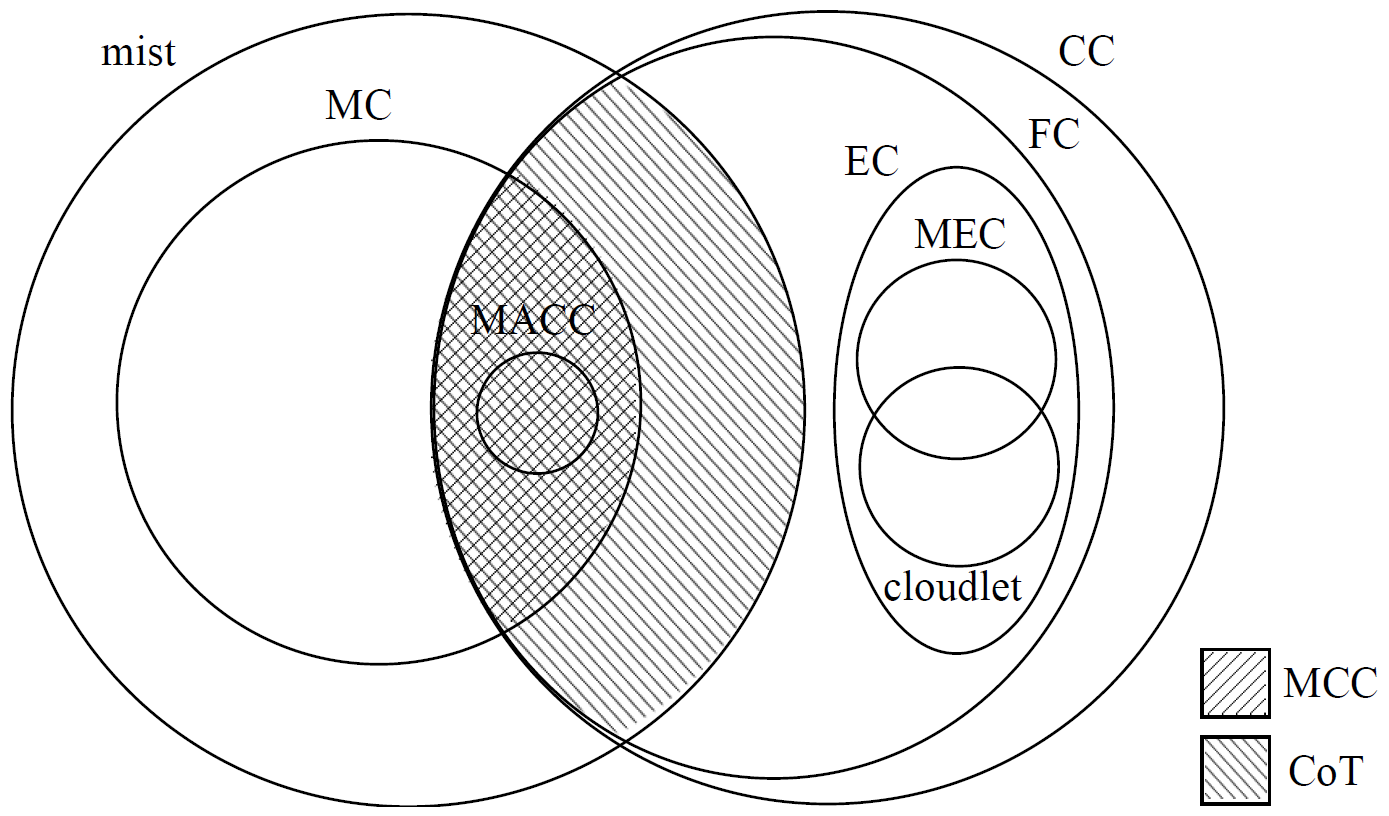
\includegraphics[width=80mm]{images/computing_paradigms}
%	\caption{A classification of scope of fog computing and its related computing paradigms (adapted from \cite{yousefpour2018all}).}
%	\label{computing_paradigms}
%\end{figure}
\begin{table}[!t]
	\scriptsize
	\begin{tabular*}{\textwidth}{l >{\centering\arraybackslash}m{0.4in} >{\centering\arraybackslash}m{0.4in} >{\centering\arraybackslash}m{0.4in} >{\centering\arraybackslash}m{0.4in} >{\centering\arraybackslash}m{0.4in} >{\centering\arraybackslash}m{0.4in} >{\centering\arraybackslash}m{0.4in} >{\centering\arraybackslash}m{0.4in} >{\centering\arraybackslash}m{0.4in}}
		\toprule
		\centering\textbf{Feature} & \textbf{CC} & \textbf{MC} & \textbf{FC} & \textbf{EC} & \textbf{MCC} & \textbf{MACC} & \textbf{MEC} & \textbf{cC} & \textbf{mist} \\[2pt]
		\toprule
		Heterogeneity support & \cmark &  & \cmark & \cmark & \cmark &  &  &  & \cmark \\ \midrule
		Infrastructure need & \cmark &  & \cmark & \cmark & \cmark &  & \cmark & \cmark & \cmark \\ \midrule
		Geographically distributed &  &  & \cmark & \cmark &  &  & \cmark & \cmark & \cmark \\ \midrule
		Location awareness &  & \cmark & \cmark & \cmark &  & \cmark & \cmark & \cmark & \cmark \\ \midrule
		Ultra-low latency &  &  & \cmark & \cmark &  &  & \cmark & \cmark & \cmark \\ \midrule
		Mobility support &  & \cmark & \cmark & \cmark & \cmark & \cmark & \cmark & \cmark & \cmark \\ \midrule
		Real-time application support &  &  & \cmark & \cmark &  &  & \cmark & \cmark & \cmark \\ \midrule
		Large-scale application support & \cmark &  & \cmark & \cmark &  &  & \cmark &  & \cmark \\ \midrule
		Standardized & \cmark & \cmark & \cmark & \cmark &  &  & \cmark &  &  \\ \midrule
		Multiple IoT Applications & \cmark &  & \cmark &  &  &  &  & \cmark & \cmark \\ \midrule
		Virtualization support & \cmark &  & \cmark &  &  &  & \cmark & \cmark &  \\ \bottomrule \\
	\end{tabular*}
	\caption{Features of fog-computing related paradigms (adapted from \cite{yousefpour2018all}).}
	\label{computing_paradigms}
	\vspace{-5mm}
\end{table}
%!TEX encoding = UTF-8 Unicode
\section{Fog Computing Architecture}
\label{sec:fog_architecture}
Fog computing is a great resource to support IoT applications' requirements in mobile environments. Taking into account what has been mentioned in Section \ref{sec:Introduction} and Section \ref{sec:Computingparadigms}, it has the following fundamental characteristics which validate the statement mentioned above (refer to Table \ref{computing_paradigms}):
\begin{itemize}[noitemsep]
	\item \textbf{Heterogeneity support}. Supports collection and processing of data of different actors acquired through multiple types of network communication, wide diversity applications and services;
	\item \textbf{Geographical distribution}. Uses anything between the cloud and \textit{things} to provide ubiquitous computing, allowing continuity of service in mobile environments;
	\item \textbf{Contextual location awareness, and low latency}. Provides low latency due to the proximity between the IoT devices and the fog nodes. Also, the contextual location allows them to be aware of the cost of communication latency with both other fog nodes and the end devices, allowing the distribution of applications across the network to be organized in a weighted manner;
	\item \textbf{Mobility support}. The exponential growth of mobile devices demands support for mobility techniques;
	\item \textbf{Real-time interactions}. Applications may involve real-time interactions rather than batch processing (e.g., as cloud does);
	\item \textbf{Scalability and agility of federated, fog-node clusters}. Fog is adaptive; may form clusters-of-nodes or cluster-of-clusters to support elastic compute, resource pooling, etc., supporting large-scale applications;
	\item \textbf{Multiple IoT applications}. Fog devices handle multiple IoT applications competing for their limited resources;
	\item \textbf{Virtualization support}. Introduces a software abstraction between the hardware and the OS and application running on the hardware;
	\item \textbf{Interoperability and federation}. Uses cooperation of different providers to support heavy applications such as real-time streaming. Moreover, it supports migration of applications to more suited fog servers depending on the current context;
	\item \textbf{Predominance of wireless access}. Most of the end devices only support wireless communication.
\end{itemize}

Nonetheless, as stated in Section \ref{subsec:Objectives}, fog still has some limitations. In order to tackle those, its overall architecture must be understood. This includes knowing: what are the actors and how they interact, how IoT nodes connect to the fog servers, how clients outsource the allocation and management of resources that they rely upon to these servers, how migration is performed, etc.

\subsection{Actors}\label{sec:fog_arch_actors}
Figure \ref{fog_architecture} shows the typical fog computing architecture. As stated before the presence of cloud servers is not imperative, however it is very important for numerous applications.\\
%, mist computing can be implemented in a layer between the fog servers and the end devices. Moreover, the presence of cloud servers is not imperative however, it is very important for numerous applications.\\
\begin{figure}
	\centering
	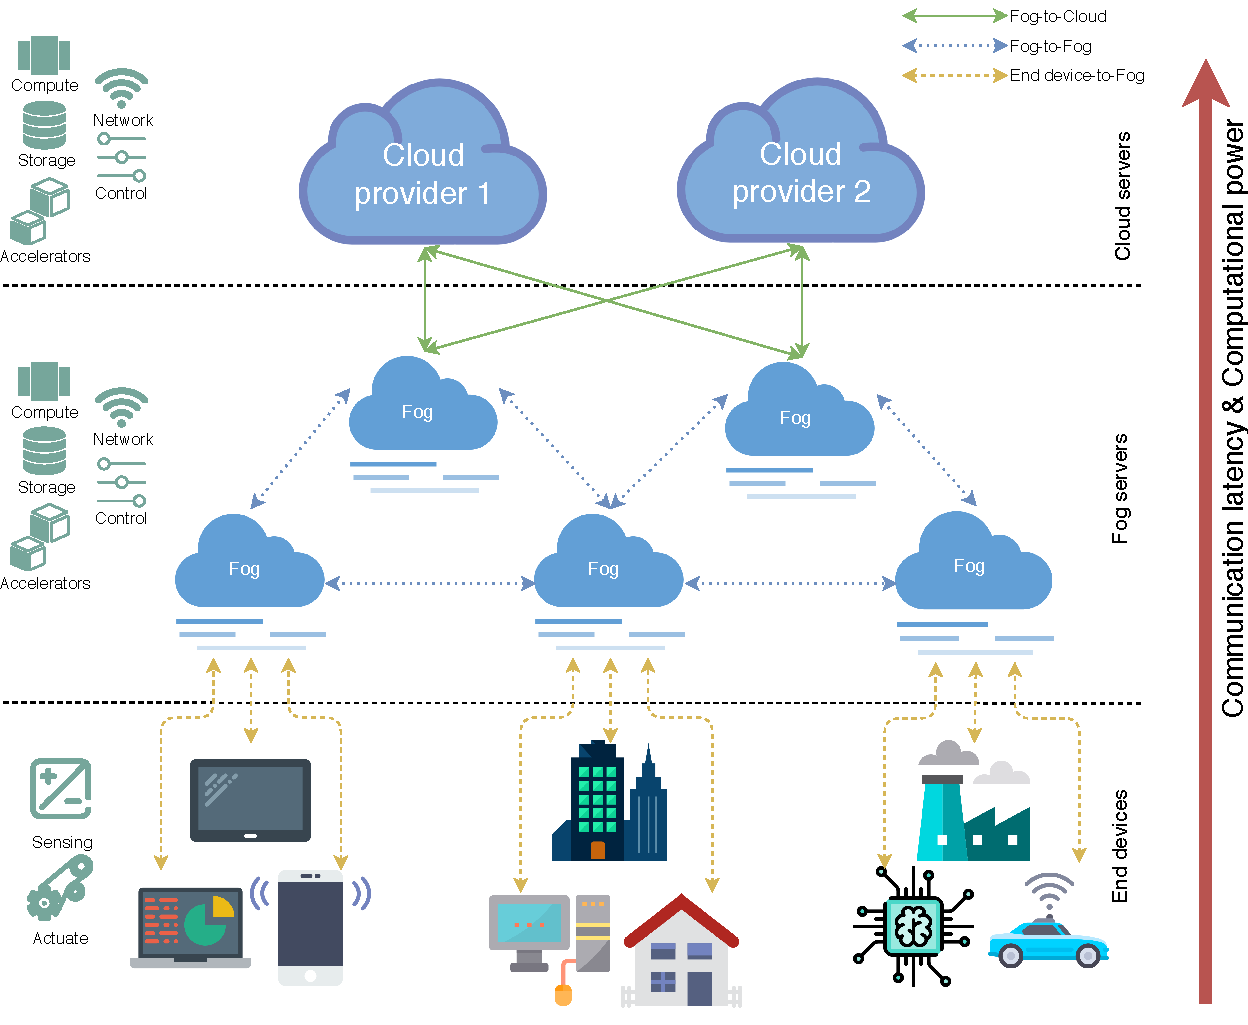
\includegraphics[width=0.60\textwidth]{images/fog_architecture/fog_architecture}
	\caption{Typical architecture of fog computing.}
	\label{fog_architecture}
\end{figure}
\noindent\tab Fog computing layer is composed by fog nodes/servers, which allow the deployment of distributed, latency-aware applications and services. Those nodes can be either physical (e.g., gateways, switches, routers, servers) or virtual (e.g., virtualized switches, virtual machines, cloudlets) components which provide computing resources to the connected end devices. When needed, they also provide network connectivity to centralized services (i.e., cloud). Moreover, fog nodes can operate in a centralized or decentralized manner or even be configured as stand-alone nodes.\\ %Therefore, they are the fundamental components in this three tier architecture (i.e., IoT-fog-cloud), being able to support the six features shown below \cite{iorga2018fog}:
%\begin{itemize}
%	\item \textbf{Autonomy}. Fog nodes can be autonomous enough to operate independently, making local decisions, at the node or cluster-of-nodes level;
%	\item \textbf{Heterogeneity}. Can be deployed in a wide variety of environments;
%	\item \textbf{Hierarchical clustering}. Fog network can be organized with an arbitrary number of layers, being able to provide different subsets of service functions while working together as a continuum;
%	\item \textbf{Manageability}. They are managed and orchestrated by complex systems that can perform most routine operations automatically;
%	\item \textbf{Programmability}. Fog nodes are inherently programmable at multiple levels, by multiple stakeholders such as network operators, domain experts, equipment providers, or end users.
%\end{itemize}
\noindent\tab Fog nodes are of most value in scenarios where data needs to be collected at the edge and where data from thousands or even millions of devices is analyzed and acted upon in micro and milliseconds \cite{openfog2017openfog}. In order to being able to support such large number of requests, especially those engaged in enhanced analytics, fog nodes may be equipped with additional hardware. Accelerators modules (refer to Fig. \ref{fog_architecture}) can be implemented to provide supplementary computational throughput. For instance, hardware accelerators can be performed through Graphics Processing Units (GPUs); they are an optimal choice for applications that support parallelism or for stream processing. Also, fog nodes may be equipped with Field Programmable Gate Arrays (FPGAs) or even Digital Signal Processors (DSPs) for this propose.\\
\noindent\tab It is worth noting that, once fog nodes can be anything with computational and storage power in the cloud-to-things continuum, the links formed in these architectures (i.e., End device-to-Fog, Fog-to-Fog and Fog-to-Cloud) can be of any type. For instance, end devices can be connected to fog servers by wireless access technologies (e.g., WLAN, WiFi, 3G, 4G, ZigBee, Bluetooth) or wired connection. Moreover, fog nodes can be interconnected by wired or wireless communication technologies, and they can be linked into the cloud by core network using fiber transmission with low-latency.\\
\noindent\tab In this architecture, the connected sensors located at the edge, generate data that can adopt two models. First, in a sense-process-actuate model, the information collected is transmitted as data streams, which is acted upon by applications running on fog devices and the resultant commands are sent to actuators. In this model, the raw data collected often does not need to be transferred to the cloud; data can be processed, filtered, or aggregated in fog nodes, producing reduced data sets. The result can then be either stored inside fog nodes or actuated upon through the actuators. Second, in a stream-processing model, sensors also send data streams, where the information mined (from the incoming streams) is stored in data centers for large-scale and long-term analytics. In this case, big data needs to be stored and does not have significant latency constraints. Being fog servers less powerful than the cloud ones, cloud is far more suited for this kind of operations. Yet, fog servers can still shrink data, doing some intermediate processing as in the previous model. This meets the aforementioned statement - although cloud is not always essential for the functioning of fog, in some applications it is beneficial or even crucial.\\
\noindent\tab The applications deployed by the connected end users into the fog nodes can be treated either as a whole or as a Distributed Dataflow (DDF) programming model, in which the applications are moduled as a collection of modules. N. Giang et al. \cite{giang2015developing} propose a DDF for IoT applications which use computing infrastructures across the fog and the cloud, allowing the application flow to be deployed on multiple physical devices rather than one. This can be particular useful to deploy less restricted modules in terms of latency to the upper fog layers (ideally to the cloud), leaving the fog nodes in the lower layers less overloaded, being able to respond faster to modules within tighter latency bounds. As already mentioned, fog utilizes virtualization mechanisms due to the numerous advantages offered. Hence, hosting an application involves creating a set of VMs or execution containers (e.g., Docker) and assign them to a set of physical or virtual components along the cloud-to-things continuum.

\subsection{Orchestration}\label{sec:fog_arch_orchestration}
When an end device needs to offload some work to a third party, it needs somehow to know where to outsource the allocation and management of resources. To do so, this architecture also needs a discovery service which concerns in finding the best available fog server, given certain capabilities and requirements. In this context, J. Gedeon et al. \cite{gedeon2017router}, propose a brokering mechanism in which available surrogates (i.e., fog nodes) advertise themselves to the broker. When it receives client requests, considering a number of attributes such as network information, hardware capabilities, and distance, it finds the best available surrogate for the client.\\
%This mechanism can be implemented on standard home routers, and thus, leverages the ubiquity of such devices in urban environments. Multiple brokers are interconnected using Distributed Hash Tables (DHTs) in order to exchange information.\\
%OK
\noindent\tab Finally, fog also needs an orchestration layer to monitor the current context in order to be able to take management decisions with regard to applications and data placement. In this context, C. Guerrero et al. \cite{guerrero2018influence} state that most of the literature considers the existence of a central broker or orchestrator gathering all system information (i.e., monitoring fog devices, clients, cloud and services), leading to poor scalability and high orchestration algorithm complexity when the number of elements is high (e.g., in smart cities). To overcome this bottleneck, O. Skarlat et al. \cite{skarlat2016resource,skarlat2017optimized} consider the concept of fog colonies. Each colony has an orchestrator and an arbitrary number of fog cells (a software component running on fog nodes). These fog cells are responsible for receiving tasks from IoT devices, and depending on the available resources, decide whether to execute it in the current fog node or to transfer it to the orchestrator. This top hierarchic element (inside a colony) will then migrate this task to the cloud or to another fog colony, if the current one is not able to handle it. The authors also state that these orchestrators could be replaced applying a decentralized approach. However, it would lead to extensive coordination and voting between the involved fog cells. On the other hand, F. Bonomi et al. \cite{bonomi2014fog} propose a distributed orchestration. This is performed implementing a Foglet software agent in each fog node. It has small footprint yet capable of monitoring machine's health and state. This information is then pushed to the distributed and persistent storage for global processing. The distributed database is also responsible for storing business policies defined by the fog administrators. The distributed policy is then embedded in every Foglet. Specifically, when a Foglet receives a request, it will gather policies from the policy repository and information relative to the currently active service instances from the services directory. With these informations, it tries to find an instance that satisfies the defined constraints. If such was found it, forwards the request, otherwise a new instance needs to be created.\\
%OK
\noindent\tab Upon the decision to migrate some application/module, service continuity is an important parameter once downtime may degrade the perceived QoS by the end user. To perform this operation, the exploited technologies are the VMs and containers. For instance, VM synthesis reduces the image size by splitting it into multiple layers, transferring only the application-specific layer which includes both the static binary program and the runtime memory data \cite{ma2017efficient}. However, this can still involve hundreds of megabytes. Also, live migration was introduced to reduce the downtime from the traditional non-live migration. The latter, suspends the VM, transfers all the content from one physical machine to another and resumes it only after the process, continuing from the same state as before suspension. In order to perform live migration there are two different approaches. On the one hand, the pre-copy memory migration firstly transfers VM’s memory state. Meanwhile, the VM keeps running. If a page gets modified (dirtied), it will be re-sent. This keeps going until either a small, Writable Working Set (WWS) has been identified, or a given number of iterations is reached. Then, the VM is suspended and sent along with the remaining dirtied pages to the target machine. On the other hand, post-copy creates and sends a snapshot of the VM state from the source physical machine to the destination, being launched at its completion. Meanwhile, during the transfer, the VM is still running in the source machine. Upon copy completion, the memory state that was kept changing is copied on demand (by page-faults) from the source to the destination machine, reducing the downtime services \cite{hines2009post}. Too many page-faults may degrade the performance of applications running inside the VM, thus pre-paging can also be used. It ensures that the next pages to be sent to the destination machine are pages in the vicinity of the last fault. Moreover, memory access patterns may also be implemented to further enhance this mechanism.\\
%OK
\noindent\tab Despite these advances, this process can be impractical in mobile fog environments due to its large size. Container represents a lighter virtualization technique. It allows developers to package up an application with all the parts needed (e.g., libraries and other dependencies). These applications share the OS of the physical machine and some libraries and/or binaries, allowing container's size to be much smaller. This eases both migration and hosting applications (i.e., more applications in a single machine and does not require restarting the OS upon migration) \cite{saurez2016incremental}.\\
%OK
\noindent\tab Nonetheless, there are two different approaches that can be exploited and implemented into the migration decisions. On the one hand, the reactive approach, as the name suggests, only performs migration when it is needed. When users and fog nodes become out of range, migration is performed to ensure QoS in mobile environments. However, I. Farris et al. \cite{farris2017optimizing} argue that downtime is not the only degrading factor of service continuity, but also the overall migration which impacts Quality of Experience (QoE) of users. On the other hand, the proactive approach deploys replicas of the user service in neighboring fog nodes (e.g., using mobility patterns). Also, periodically the state in these nodes is updated. The main goal is to reduce the migration time and improve QoE. However, this approach brings new costs at different levels such as computation, memory, and networking.\\
%For this propose, E. Saurez et al. \cite{saurez2016incremental} propose foglets, a programming model that facilitates distributed programming across fog nodes. It is implemented through container-based visualization. Foglets not only provides APIs for application development as DDFs, including the primitives for communication between the application components, but also embodies algorithms for the discovery and incremental deployment of resources commensurate with the application needs. Moreover it provides mechanisms for QoS-sensitive and workload sensitive migration of application components due to end devices mobility and application dynamism. Specifically, there are four entities in the foglets runtime system: the discovery server, the docker registry server, the entry point daemon, and the worker process. The discovery server is a partitioned name server that maintains a list of fog nodes available. Docker registry server is a server that contains the binaries for the applications that have been launched on the foglets infrastructure. The entry point daemon executes directly on top of the host OS in the fog node, awaits requests and periodically sends ``I am alive'' message to the discovery server. Finally the worker process carries out the functionality contained in a particular application component assigned to it.\\
\noindent\tab Fog servers can provide reduced latencies and help in avoiding/reducing traffic congestion in the network core. However, this comes at a price: more complex and sophisticated resource management mechanisms are needed. This raises new challenges to be overcome such as dynamically deciding when, and where (device/fog/cloud) to carry out processing of requests to meet their QoS requirements. Furthermore, in mobile environments such mechanisms must incorporate mobility (i.e., location) of data sources, sinks and fog servers in the resource management and allocation process policies to promote and take advantage of proximity between fog and end devices.
%!TEX encoding = UTF-8 Unicode
\section{Migration Optimization in Mobile Fog Environments}
\label{sec:Migration}
When an IoT device needs to offload some heavy application to a third party, ideally it will be connected to the nearest server, securing a hop away fog server to ensure the shortest network delay. However, as their physical distance increases either by device or server movement, their network distance (i.e., the number of hops) will also increase. Hence, both latency and bandwidth usage by the intermediate links will increase, resulting in poor connectivity. This away, in such dynamic environments the decision-making of where to offload the work is a major concern. Moreover, even if both clients and servers are static, the end-to-end latency may increase due to unexpected crowds of mobile clients seeking to connect or making requests to the same fog server simultaneously, which may lead to QoS violations.\\
\noindent\tab In Section \ref{sec:fog_architecture} it was discussed that applications can be offloaded as a whole, or as a set of modules which may have different latency constraints. Regardless of their type, whenever it is justified the system needs to be readjusted. This is performed through the exchange of VMs or containers (containing the applications or modules) between fog nodes. For this reason, it is necessary to answer the following questions: \textit{When is this exchange justified? And what is the best placement for those applications and/or modules?} As stated in Section \ref{subsec:Objectives}, this work intends to implement multi-objective management decision-making in a novel architecture. Hence, this state-of-the-art section intends to study some proposed mechanisms in the literature.

\subsection{QoS-Aware}\label{sec:QoS}
The first objective that fog computing has to guarantee is QoS. When users outsource some delay constrained task or application, they expect fog to be adaptive enough so that they can move while their time boundaries are met. Without this objective fog computing is useless once it appears, in part, to help cloud computing to overcome this limitation.\\
%OK
\noindent\tab In this context, the work performed by T. Rodrigues \cite{rodrigues2017pso} et al. is focused on increasing the QoS offered to its users by lowering both transmission and processing delays.
%On the one hand, the transmission delay encompass the time spent to send the data/task to the cloudlet and the time interval to receive the results. On the other hand, processing delay regards to the time that the work spends in the cloudlet's work queue and the respective time to being processed.
Their goal is achieved by finding the best placement of each mobile user's VM. They assume that each user is connected to the cloudlet which offers the best Received Signal Strength (RSS), that, in turn, is also responsible for hosting its VM. Therefore, their goal is to compute the optimal transmitting power for each cloudlet which will control the RSS and, consequently, change user connections. In order to optimize the formulated problem, is applied a Particle Swarm Optimization (PSO) model. Their architecture assumes the presence of a central unit which is responsible for collecting the physical locations of users and cloudlets and then to execute the model. It is worth noting that when any user changes its connection (i.e., connects to another cloudlet), its VM is also migrated, however this delay is not considered. Also, their work considers that each VM task arrival rate follows a Poisson process with the same rate for all users and does not specify what is the algorithm optimal frequency of execution.\\
%OK
\noindent\tab The study performed by X. Sun et al. \cite{sun2016primal} presents, a case scenario where the end devices are mobile. To perform this work they use a cloudlet network architecture to bring the computing resources from the centralized cloud to the edge. They present the PRofIt Maximization Avatar pLacement (PRIMAL) strategy. PRIMAL maximizes the trade-off between the migration gain (i.e., the end-to-end delay reduction) and the migration cost (i.e., the migration overheads incured in the avatar, which compromise its performance), by migrating the avatars (a software clone located in a cloudlet) to their optimal locations, using  pre-copy live migration. To solve the formulated problem, they use the Mixed-Integer Quadratic Programming tool in the CPLEX solver to find the heuristic solution of PRIMAL. It is worth noting that the considered gain only considers the end-to-end delay reduction between the user's base station and user's avatar. Both gain and cost do not consider the servers state nor network state. \\
%R. Urgaonkar et al. \cite{urgaonkar2015dynamic} argue that because of the uncertainty in user mobility and request patterns, it is challenging to make migration decisions in an optimal manner. Also, in this work is argued that methods which depend on mobility patterns have several drawbacks, namely: (1) they require extensive knowledge of the statistics of the user mobility and request arrival processes that can be impractical to obtain in a dynamic network, (2) even when this is known, the resulting problem can be computationally challenging to solve, and (3) any change in the statistics would make the previous solution suboptimal and would require recomputing the optimal solution. Thus, they propose a new model, inspired by the technique of Lyapunov optimization, that overcomes these drawbacks (i.e., does not require any knowledge of the transition probabilities). The overall problem of dynamic service migration and workload scheduling to optimize system cost while providing end user performance guarantees is formulated as a sequential decision-making problem in the framework of Markov Decision Processes (MDPs). The cost depends on reconfiguration cost, inherent to migration services (i.e., moving the application from one cloudlet to another) and on transmission cost (i.e., time-average of user-to-cloudlet request routing) which depends on their distance. Their goal is to design a control algorithm for making request routing decisions so that the time-average overall transmission and reconfiguration costs are minimized while serving all requests with finite delay. They have developed a new approach for solving a class of constrained MDPs that possess a decoupling property. When this property holds, their approach enables the design of simple online control algorithms that do not require any knowledge of the underlying statistics of the MDPs.

\subsection{Bandwidth-Aware}\label{sec:bandwidth}
Minimization of network utilization is one of the main objectives of fog computing. In fact, fog appears to overcome this inherent limitation of cloud computing. Thus, aside from ensuring QoS, it is also important to reduce bandwidth usage.
%Thus, besides guarantee QoS, it is also  important to reduce bandwidth usage.
This utilization of network is essentially due to three factors: the transmission of virtualized resources (VMs or containers) which contain the applications/modules, transmission of data between the end device and the deployed application into the fog nodes, and control messages exchanged between fog nodes. If the applications are deployed using DDF programming model a fourth factor rises, the data transmission between modules. In this section, the reviewed literature propose models to mitigate bandwidth usage providing long-term QoS, reducing the number of migrations.\\
%
\noindent\tab B. Ottenwälder et al. \cite{ottenwalder2013migcep} consider an environment with mobile devices and fixed fog nodes, where users offload real-time applications such as Complex Event Processing (CEP). CEP is a paradigm where changes in sensor measurements are modeled as events, while the application is modeled as set of event-driven operators. They state that each migration comes with a cost, consequence of the local state that also needs to be migrated along with the operators. Thus, frequent migration would significantly decrease the system performance. To overcome this limitation, they propose a placement and migration method for fog providers to support operator migrations in Mobile Complex Event Processing (MCEP) systems. Their method plans the migration ahead of time through knowledge of the MCEP system and predicted mobility patterns towards ensuring application-defined end-to-end latency restrictions and reducing the network utilization. These predicted mobility patterns were captured using three different methods: uncertain locations from the \textit{dead reckoning} approach (linear), certain locations that could stem from a \textit{navigation} system (navi), and \textit{learned} transitions between leaf broker (learned). This method allows a minimization of migration costs by selecting migration targets that ensure a low expected network utilization for a sufficiently long time.\\ %Moreover, they present how the application knowledge of the CEP system can be used to improve current live migration techniques for VMs to reduce the required bandwidth during the migration (i.e., unnecessary events are not migrated).\\
%OK1
\noindent\tab Also in this context, W. Zhang et al. \cite{zhang2016segue} state that previous studies have proposed a static distance-based MDP for optimizing migration decisions. However, these models fail to consider dynamic network and server states in migration decisions, assuming that all the important variables are known. Moreover, they also point out another unaddressed problem which lies in the recalculation time interval of the method. Since running MDP is a heavy computing task, a short recalculation interval introduces a considerable overhead to the server. On the other hand, a long recalculation interval may translate into lazy migration, resulting in periods of transgression of QoS guarantees. In order to overcome these issues, the authors propose SEGUE. This model achieves optimal migration decisions by providing a long-term optimal QoS to mobile users in the presence of link quality and server load variation. Additionally, SEGUE adopts a QoS aware scheme to activate the MDP model. In other words, it only activates the MDP model when QoS violation is predicted. Thus, it avoids unnecessary migration costs and bypasses any possible QoS violations while keeping a reasonable low overhead in the servers.
%The QoS prediction module assumes that mobile location, follows a mobility pattern with only one dimension.
The problem formulation is then formulated as a cost-reward between the predicted long term QoS improvement and the service downtime.\\
%The work performed by Wuyang Zhang et al. \cite{zhang2017towards} use as case study the Massively Multiplayer Online Gamse (MMOGs) with Virtual Reality (VR) technologies, VR-MMOGs. They present the main challenges of VR-MMOGs, namely: stringent latency, high bandwidth, and large scale requirements. This work shows one problem that remains unsolved: how to distribute the work among the user device, the fog nodes, and the center cloud to meet all three requirements especially when users are mobile. Their approach was to place local view change updates on fog nodes for immediate responses, frame rendering on fog nodes for high bandwidth, and global game state updates on the center cloud for user scalability. In this kind of game, users need to move, so in order to keep a low latency communication, they also propose an efficient service placement algorithm based on MDP. This method takes into account the presence of dynamic network states and server workload states, and user mobility providing long-term QoS. To ensure feasibility of this method, they come up with an approach that reduces the algorithm complexity in both storage and execution time. Nonetheless, unlike many of the service migration solutions which assumes an ignorable service transition time, they point out that it is impossible to migrate a fog service from one fog to another instantly given the size of a VR game world. Therefore, they propose a mechanism to ensure a new fog node is activated when a player connects to the new one.
%\\ \textit{Concluding Remarks} - The presented literature intends to reduce the number of migrations by providing long term QoS. This also reduces the downtime service, increasing QoS. While the first work, considers distributed applications, where the set of operators which are deployed among a set of fog nodes need some coordination in migrations, the rest consider applications as a whole. As already discussed, DDF programming model can bring advantages to fog computing. However the two latter works consider network state and server performance (resulting in workload) in their models. They all fail in not consider an energy consumption, a cost model and an environment where fog nodes can be movable.

\subsection{Energy-Aware}\label{sec:energy}
In order to achieve the QoS objective, the placement of applications and their modules has often to be moved between different entities that compose the things-fog-cloud architecture which evolves energetic costs (both in terms of processing and communication). For instance, it is needed to exchange control messages, communicate between modules placed at different nodes, change the module placement, etc. Thus, energy-aware must be an important factor to be taken into account in the decision making algorithm of \textit{when} and \textit{where} to offload work to another entity in order to minimize fog infrastructure providers' cost.\\
%OK1
\noindent\tab In this context, R. Deng et al. \cite{deng2016optimal} focused on investigating system power consumption and network delay trade-off in cloud-fog services. They formulate a workload allocation problem, which suggests the optimal workload allocations between fog and cloud toward the minimal power consumption with the constrained service delay. This was performed through the modeled power consumption and delay functions of each part of the fog-cloud computing system. It is worth noting that power consumption only considers energy consumption of work computation, disregarding communication costs. The problem is then tackled using an approximate approach through decomposition, and formulation of three subproblems, being solved through existing optimization techniques. This work also does not considers dynamic environments. All variables are static including the position of fog nodes and end devices. Also there is no cooperation between fog nodes and the communication delay between a fog node and a cloud server is only characterized by its latency, ignoring the bandwidth. Similarly to the majority of the presented works, the decision-making is performed in a centralized manner.\\
%OK1
\noindent\tab Y. Xiao et al. \cite{xiao2017qoe} investigate two performance metrics for fog computing networks: the QoS of mobile users and the power efficiency of fog nodes. In their scheme, fog nodes can process or offload to other fog nodes part of the workload that was initially sent to the cloud. Fog nodes decide whether to offload the workload to neighbors or locally process it, under a given power constraint. A distributed optimization algorithm based on Alternating Direction Method of Multipliers (ADMM) via variable splitting is proposed. This allows to achieve the optimal workload allocation solution that maximizes QoS of users under the given power efficiency. In this work, power efficiency of each fog node is measured by the amount of consumed energy to offload each unit of workload from the cloud. Note that their work do not use the concept of VMs nor DDF programming model, and the considered environment is static (i.e., nodes and clients are static), avoiding the inherent migration problems.
%\noindent\tab C. Anglano et al. \cite{anglano2018profit} present the Online Profit Maximization (OPM) algorithm. It is an approximation algorithm that aims to increase fog infrastructure providers' profit, by reducing the overall energy consumption of the infrastructure without a priori knowledge, and yet guarantee the QoS to its mobile end users. This cost is the sum of energy costs inherited from the execution of applications, cloning and migrating the VMs, turning on and off the fog nodes, and monetary penalties for QoS violations. To solve the formulated problem, their work applies an online optimization algorithm in each recalculation time interval, achieving near optimal solutions.\\(TEM CLONES E DEVIA ESTAR NO CUSTO)
%\noindent\tab The work performed by A. Kattepur et al. \cite{kattepur2016resource} investigates the problem of computation offloading in fog computing. They present an energy model and communication costs with respect to computational offloading and formulate an optimal deployment strategy when dealing with distributed computation, while keeping energy and latency constraints in mind. The formulations are solved in Scilab using the Karmarkar linear optimization solver. They evaluate their approach in a sense-process-actuate model using a network of mobile robotic sensor-actuators developed in Robot Operating System (ROS)/Gazebo.(PEERS ROBOT/FOG NODE)\\
%OK1
\subsection{Cost-Aware}\label{sec:cost}
As aforementioned, besides guarantying QoS to its users, fog service providers also need to maximize their profit. Hence, it is important to develop an accurate cost model in order to accept and implement fog computing. Besides, similarly to what cloud does, fog has to implement a pay-as-you-go cost model in order to provide services on-demand to its users, without under- or over-provisioning, and charging a fair price. To this end, the cost model needs to apply a communication model, an energy model, and a resource utilization model.\\
%OK1
\noindent\tab In this context, L. Gu et al. \cite{gu2017cost} state the importance of fog computing in medical cyber-physical systems as the number of users grows. They state that different infrastructure service providers may apply different charging policies. Therefore, in this paper, the authors aim to minimize the overall resource management cost while satisfying the QoS requirements. They formulate the cost minimization problem in a form of Mixed-Integer NonLinear Programming (MINLP) with joint consideration of communication BS association, subcarrier allocation, computation BS association, VM deployment and task distribution. To tackle the high computational complexity of solving this problem, they linearize it into a Mixed-Integer Linear Programming (MILP) problem. This way they are able to solve the optimal programming model using solvers such as CPLEX and Gurobi. However, it is still time-consuming due to the existence of many integer variables. To this end, they further propose an LP-based two-phase heuristic algorithm. It is worth noting that this work explores placement of VMs in fog computing, whereas it does not tackle this problem in mobile environments, disregarding both users and servers mobility, consequently not addressing the inherent migration problems. Moreover, the proposed method to verify if the QoS requirements are met do not consider the servers state nor network state.\\
%OK1OK
\noindent\tab O. Skarlat et al. \cite{skarlat2017optimized} start by describing a conceptual framework for resource provisioning and service placement in fog. They consider the concept of fog colonies (refer to Section \ref{sec:fog_arch_orchestration}) using a cooperative execution of IoT applications (DDF programming model). Based on this concept, their work, formalizes an optimization problem that aims to adhere to the deadlines on deployment and execution time of applications and to maximize the utilization of existing resources in fog, rather than in cloud, leading to lower execution cost. To solve this placement problem, they apply different approaches, namely the exact optimization method and its approximation through a greedy first fit heuristic and a Genetic Algorithm (GA). They also compare the results, in the fog simulation toolkit iFogSim, to a classical approach that neglects fog resources and runs all services in a centralized cloud. The goal of the evaluation is to identify the best approach to solve the proposed optimization problem in terms of resulting QoS, QoS violations, and cost. The latter is composed only by the execution costs in cloud infrastructures, neglecting execution costs in fog nodes. Their work does not provide mobility mechanisms, not addressing the inherent migration problems. Moreover, all the communications within each fog colony need to be performed through the respective fog orchestration control, introducing new non-negligible communication latencies. Also, the proposed method to verify if the QoS requirements are met do not consider the servers state nor network state.\\
%OK1
\noindent\tab The work performed by T. Bahreini et al. \cite{bahreini2017efficient} also addresses multi-tier placement (DDF programming model). The authors formulate the Multi-Component Application Placement Problem (MCAPP). Their objective is to find a mapping between components and servers, such that the total placement cost is minimized. This cost is composed of four types of costs at each time slot: (1) the cost of running one component in a specific server, (2) cost of relocating one component from one server to another, (3) communication cost between one component and the user, and (4) communication between components. With the objective to minimize the overall cost incurred when running the application, they formulate the offine version of the problem as a Mixed Integer Linear Program (MILP) and then developed a heuristic algorithm for solving the online version of the problem. The algorithm is based on an iterative matching process followed by a locals search phase in which the solution quality is improved. This way they use simple algorithmic techniques, avoiding complex approaches such as those based on MDPs. They state that the proposed algorithm has low complexity and adds a negligible overhead to the execution of the applications. Although this work considers the location of servers in the estimation of costs (2) through (4), it does not consider an environment with mobile fog nodes. Also, it only considers the presence of only one user with only one application. Moreover, in each time slot, each server is used by at most one component, not properly taking advantage of fog computing.\\
%
\noindent\tab A different approach was taken by D. Ye et al. \cite{ye2016scalable}. They leverage the characteristics of buses and propose a scalable fog computing paradigm with servicing offloading in bus networks. Knowing that buses have fixed mobility trajectories and strong periodicity, they consider a fog computing paradigm with service offloading in bus networks which is composed by roadside cloudlets and bus fog servers. The roadside cloudlet consists of three components: dedicated local servers, location-based service (LBS) providers, access points (APs). The dedicated local servers virtualize physical resources and act as a potential cloud computing site. LBS providers offer the real time location of each bus in bus networks. APs act as gateways for users and bus fog servers within the communication coverage to access the roadside cloudlet. As cloudlets have limited computational and storage resources, they may become overloaded. The bus fog server is a virtualized computing system on bus, which is similar to a light-weight cloudlet server. Hence, those buses not only provide fog computing services for the users on bus, but also are motivated to accomplish the computation tasks offloaded by roadside cloudlets. This allocation strategy is accomplished using GA, where the objective is to minimize the cost that roadside cloudlets spend to offload their computation tasks. Note that there is only considered mobility of fog nodes (i.e., users are static). Also, their problem assumes the applications are deployed as a whole, not addressing the DDF programming model advantages and difficulties in fog computing. Nonetheless, the proposed method to verify if the QoS requirements are met do not consider the servers state nor network state. 
%Although this work refers to mobile users, its meaning is not literal (representing the workload of both buses and cloudlets), being supported only the mobility of fog servers.

\subsection{Multi-Objective}\label{sec:multi}
In some cases rather than only one objective, it might be indispensable to improve the system performance from several perspectives/objectives. However, those can be independent and conflicting objectives. Therefore, unlike the previous sections, the current one aims to present works that were intended to study multi-objective migration optimization algorithms.\\
\noindent\tab Y. Nan et al. \cite{nan2017adaptive} aim to provide an energy-efficient data offloading mechanism to ensure minimization of long-term system cost (measured by the money spending on energy consumption) and yet guarantee that users do not perceive a poor QoS. Their work assumes that fog nodes have two sources of energy. The primary source is the solar or green energy which has no monetary cost, however it is finite (in each time slot, the volume of electricity converted from solar energy is a stochastic value depending on the weather conditions). As a backup energy supply, fog nodes have also access to the non-free grid or brown power supply. In addiction, they also assume the presence of cloud data centers which, in this case, have only access to the grid power supply. Their work describes an online adaptive algorithm, Lyapunov Optimization on Time and Energy Cost (LOTEC). LOTEC is a quantified near optimal solution and is able to make control decision on application offloading by adjusting the two-way trade-off between average response time and average cost. This decision-making distributes the incoming applications to the corresponding tiers without a priori knowledge of users and system status. Note that, in this work, there are no VM support nor DDF programming model. Also, there is no fog cooperation and both users and fog nodes are static, not addressing the inherent problems of migration.\\
%OK1
\noindent\tab The work performed by L. Yang et al. \cite{yang2016cost} aim to minimize both the average latency of all the users’ request loads and the overall costs of service providers. The latter is composed by minimization of both resource usage on cloudlets and service placement transitions. The authors state that this three-way trade-off is a difficult problem. Moreover, the request load could vary significantly and frequently in both spatial and temporal domain due to the mobility of users. Such dynamic request load implies a periodic update of decisions, keeping in mind both the current performance and the expected future workload (using user’s mobility pattern and services access pattern to predict the distribution of user’s future requests). In order to solve this three way trade-off, the authors first formulate the snapshot problem, named Basic Service Placement Problem (BSPP), which aims to optimize the access latency with the capacity constraints of cloudlets. As it is hard to solve, they design a competitive heuristic to BSPP which outperforms a set of benchmark algorithms. Their work further extends BSPP in order to minimize the above three-way trade-off. To do so, they normalize the costs and apply a weighted sum, allowing the formulation of a single objective problem. It is worth noting that this work does not consider DDF programming model, energy and bandwidth models, routing problems nor mobility of fog nodes.\\
%OK1
\noindent\tab L. Wang et al. \cite{wang2018service} address the social VR applications to study the problem of placing VMs deployed in fog environments such that, the total cost in the overall cost in the fog system is minimized. Although motivated by VR applications, the authors state that this problem is fundamental for any applications that require interactions between either mobile user and the respective VM or user and VMs of other users. The placement problem is to decide where to place the service entity of each user among the cloudlets in order to achieve economic operations of cloudlets as well as QoS. This problem is non-trivial due to the following challenges: (1) cloudlets are heterogeneous in terms of activation and running costs, (2) VMs need to exchange metadata frequently with the associated users and other VMs (of other users), and (3) due to the fact that cloudlets are not intentionally designed to simultaneously accommodate many VMs, especially for VR applications where specific hardware such as GPU may be involved, resource contention needs to be controlled. The authors model the aforementioned challenges with four types of cost: activation cost, the placement cost, the proximity cost, and the collocation cost. These costs are then formulated as a single objective problem by using a weighted sum. They formulate the problem as a combinatorial optimization, which is NP-hard. To solve the problem, they propose ITerative Expansion Moves (ITEM) algorithm, a novel algorithm based on iteratively solving a series of minimum graph cuts. The algorithm is flexible and is applicable in both offline/static (i.e., no movement) and online/dynamic (i.e., with users mobility) scenarios. It is worth noting that the concept of DDF is not applied in this work nor considers fog nodes mobility.\\
%OK
\noindent\tab Motivated by the trade-off between local execution power consumption and the offloading delay, the work performed by L. Liu et al. \cite{liu2018multiobjective} has the objective of minimize energy consumption, delay, and payment cost (E\&D\&P) for mobile devices in fog computing environments, using queuing theory. Specifically, three types of queues are applied, namely: mobile devices are considered as a M/M/1 queue, fog node as a M/M/c queue with a defined maximum request rate, and cloud as a M/M/$\infty$ queue. Both wireless transmission and computing capabilities are explicitly and jointly considered when modeling this three-way trade-off. They formulate the optimization problem by finding the optimal offloading probability and transmit power. Using the scalarization method, they were able to transform the multi-objective into a single-objective optimization problem. In order to solve that single-objective problem they proposed an Interior Point Method (IPM)-based algorithm which can reduce the accumulated error and improve the calculation accuracy during the iteration process effectively. Note that, in the considered system, there is no movement and there exists only one fog node, which does not fulfill the ubiquity characteristic of fog computing.\\
%OK
\noindent\tab L. Wang \cite{wang2018moera} et al. address two categories of costs, namely: static, which includes the operation cost and the service quality cost, and dynamic, comprising the reconfiguration cost and the migration cost. While the former is independently incurred inside each time slot, the latter is only charged for decision transitions across consecutive time slots. Operation cost refers to the incurred cost in terms of resources utilization (i.e., Central Processing Unit (CPU) and memory) or energy in each cloudlet. Service quality cost, which aims to capture the user perceived QoS, is proportional to the network delay between the user and its workload which may be distributed over several cloudlets. Reconfiguration cost regards to the increase of workload across time slots in each cloudlet. Finally, the migration cost includes both bandwidth cost on the network and the migration delay (both moving out of and into each cloudlet). The single objective problem formulation takes into account all these costs using a weighted sum.
%It is observed that, if all inputs were given in advance (operation prices and the user mobility patterns in all time slots), this problem could be solved using a linear program solver. However, this is impossible in the online setting, where the input data are revealed step-by-step over time.
They propose Mobility-agnostic Online Edge Resource Allocation (MOERA) based on the ``regularization'' technique, which decomposes the problem into subproblems and solve them using convex programming. This algorithm receives as input the user’s workload and location and decides how resources should be allocated, such that the workload demands from every user is fulfilled while the overall cost system is minimized. Note that their work do not consider the DDF programming model, avoiding its advantages and difficulties in fog computing, and all fog nodes are static.
%Note that although service quality cost intends to capture and minimize user perceived QoS, it only considers the latency between the user and its workload, however QoS should also take into account both network and server state.

\subsection{Concluding Remarks}
The presented literature addresses different objectives regarding optimization in fog environments. For instance in Section \ref{sec:QoS}, the conferred works perform a single objective optimization in order to minimize the QoS offered to the end users. The works in Section \ref{sec:bandwidth}, Section \ref{sec:energy} and Section \ref{sec:cost}, also perform a single objective optimization, however, besides taking into consideration the QoS, they also consider bandwidth usage, energy and cost, respectively. In Section \ref{sec:multi} were presented works that combine, in a multiple objective optimization, some of the above mentioned objectives.\\
\noindent\tab For the sake of analysis between the works described above, Table \ref{tab:literature:features} presents a comparison of the features supported, and Table \ref{tab:literature:problem} compares the problem formulation, from whose perspective the problem is being optmized, as well as the algorithm(s) implemented in order to solve the problem formulation.\\
\noindent\tab Although their approaches contribute to the improvement of fog computing, they do not account all the aspects that this work aims to cover. Regarding Table \ref{tab:literature:features} it is noticeable that there is lack of support for using DDF programming model. As already discussed, in Section \ref{sec:fog_arch_actors}, it can bring advantages to fog computing. Also, some works do not support the use of VM, considering, in this case, only the workload that needs to be processed. However, as previously mentioned, in Section \ref{sec:fog_architecture}, one of the main goals of fog computing is to support running multiple IoT applications at the same time. To do so, it is mandatory to use some kind of virtualization technique as discussed in Section \ref{sec:Introduction}.
%only one application with multiple users performing request to it. As previously mentioned, in Section \ref{sec:fog_architecture}, one of the main goals of fog computing is to support running multiple IoT applications at the same time.
It also is clear that the analyzed works fail to consider a fully dynamic environment. Even though some take into account mobility either from the mobile devices or fog nodes, none of them acknowledges both simultaneously. Migration is also a challenge little explored. However, due to the fact that the environments in which the fog is used are not static, it is crucial in order to rearrange the placement of applications or modules whenever needed. Finally, in order to improve the system flexibility, the presence of multiple fog nodes and the cooperation between them is also essential, however, this is not considered in some cases. \\
\noindent\tab With respect to the optimization problem, Table \ref{tab:literature:problem}, there are several approaches. 
%These works aim to optimize their formulated problem from different perspectives, including: the fog provider which may request resources form a cloud provider, the system provider (i.e., cloud and fog provider), the fixed fog provider which may request resources form a mobile fog provider, the service provider or broker which may request resources from several fog and/or cloud providers in order to allow users to use its service, and finally the mobile devices perspective which may also request resources from several fog and/or cloud providers.
These works aim to optimize their formulated problem from different perspectives. The fog provider perspective owns a fog infrastructure which may request resources form a cloud provider. The system provider assumes the ownership of both fog and cloud infrastructures. The fixed fog provider (special case of fog provider) perspective assumes only the possession of the fixed fog infrastructure. The service provider or broker as the name suggests wants to provide a service to its users, however is owns any physical infrastructure. Finally the mobile devices perspective is similar to the service provider in the sense that needs to request resources from other fog and/or cloud providers, however, in this case, the objectives refer to the mobile devices (e.g., minimize the energy consumption of mobile devices).\\
\noindent\tab Independently from the optimization perspective, we consider that there are some flaws in the reviewed literature. First, in order to support real-time IoT applications, its demands in terms of response deadline should always be a constrain. For instance, if we consider a hard real-time application (e.g., autonomous car controller), in the worst case scenario each deadline have to be guaranteed to be fulfilled. In this regard, it is mandatory to take into account the state of servers and links, however, as aforementioned, most of the works which define QoS constrains do not take these parameters into consideration. Note that the works performed in \cite{deng2016optimal} and \cite{nan2017adaptive} were able to compute the QoS by taking into account these parameters because there work considers no fog cooperation (i.e., the path is always client-fog-cloud). Similarly the work performed in \cite{ottenwalder2013migcep} was also capable to do it, however, as there were fog cooperation, the key element was to know each data and migration routing. Finally, the work \cite{zhang2016segue} also considers these parameters, however, in this case, those were captured with their refined hybrid push/probe technique which introduces some overhead to the system.
From a similar perspective, users may also demand a maximum time to migrate its service due to service degradation during this period. As shown, in Table 2, none of the reviewed works has addressed this issue. Finally, some works do not consider the amount of resources each node can provide (i.e., CPU, memory and storage) and/or do not consider the amount of bandwidth available in the links. As aforementioned, in Section \ref{sec:fog_arch_actors}, nodes can be anything with computational and storage resources and the communications can also be of any type. This way, those constrains should always be accomplished in order to ensure the solution found do no exceed the available resources.\\
\begin{table}
	\caption{Features comparison of the above described works.}
	\scriptsize
	\begin{tabular}{
			>{\arraybackslash}m{0.32in}
			>{\centering\arraybackslash}m{0.41in}
			>{\centering\arraybackslash}m{0.41in} >{\centering\arraybackslash}m{0.41in} >{\centering\arraybackslash}m{0.41in}
			>{\centering\arraybackslash}m{0.41in}
			>{\centering\arraybackslash}m{0.41in}
			>{\centering\arraybackslash}m{0.41in} >{\centering\arraybackslash}m{0.41in}
			>{\centering\arraybackslash}m{0.41in} >{\centering\arraybackslash}m{0.41in}
		}
		\toprule
		Ref. &
		VM support&
		Multiple VM server support&
		DDF&
		Multiple fog nodes&
		Fog cooperation&
		Cloud server&
		Users mobility&
		Fog servers mobility&
		Location aware&
		Migration\\
		\toprule
		\cite{rodrigues2017pso} & \cmark & \cmark & & \cmark & \cmark & & & & \cmark & \cmark \\
		\midrule
		\cite{sun2016primal} & \cmark & \cmark & & \cmark & \cmark & & \cmark & & \cmark & \cmark \\
		\midrule
		\cite{ottenwalder2013migcep} & \cmark & \cmark & \cmark & \cmark & \cmark & \cmark & \cmark & & \cmark & \cmark \\
		\midrule
		\cite{zhang2016segue} & \cmark & \cmark & & \cmark & \cmark & & \cmark & & \cmark & \cmark \\
		\midrule
		\cite{deng2016optimal} & & & & \cmark & & \cmark & & & & \\
		\midrule
		\cite{xiao2017qoe} & & & & \cmark & \cmark & \cmark & & & & \\
		\midrule
		\cite{gu2017cost} & \cmark & \cmark & & \cmark & \cmark & & & & \cmark & \\
		\midrule
		\cite{skarlat2017optimized} & \cmark & \cmark & \cmark & \cmark & \cmark & \cmark & & & & \\
		\midrule
		\cite{bahreini2017efficient} & \cmark & & \cmark & \cmark & \cmark & \cmark & \cmark & & \cmark & \cmark \\
		\midrule
		\cite{ye2016scalable} & \cmark & \cmark & & \cmark & \cmark & & & \cmark & \cmark & \\
		\midrule
		\cite{nan2017adaptive} & & & & \cmark & & \cmark & & & & \\
		\midrule
		\cite{yang2016cost} & \cmark & \cmark & & \cmark & \cmark & \cmark & \cmark & & \cmark & \cmark \\
		\midrule
		\cite{wang2018service} & \cmark & \cmark & & \cmark & \cmark & & \cmark & & \cmark & \cmark \\
		\midrule
		\cite{liu2018multiobjective} & & & & & & \cmark & & & & \\
		\midrule
		\cite{wang2018moera} & \cmark & \cmark & & \cmark & \cmark & & \cmark & & \cmark & \cmark \\
		\bottomrule
	\end{tabular}
	\label{tab:literature:features}
\end{table}
\begin{table}
	\caption{Problem comparison of the above described works.}
	\scriptsize
	\begin{tabular}{
			>{\arraybackslash}m{0.15in}
			>{\centering\arraybackslash}m{0.88in} >{\centering\arraybackslash}m{0.08in} >{\centering\arraybackslash}m{0.08in} %>{\centering\arraybackslash}m{0.08in}
			>{\centering\arraybackslash}m{0.08in} >{\centering\arraybackslash}m{0.08in} >{\centering\arraybackslash}m{0.08in} >{\centering\arraybackslash}m{0.08in} >{\centering\arraybackslash}m{0.08in} >{\centering\arraybackslash}m{0.08in} >{\centering\arraybackslash}m{0.08in} >{\centering\arraybackslash}m{0.08in}
			>{\centering\arraybackslash}m{0.08in} >{\centering\arraybackslash}m{0.08in} >{\centering\arraybackslash}m{0.6in}
			>{\centering\arraybackslash}m{1in}
		}
		\toprule
		& & \multicolumn{4}{c}{Objectives} &
		\multicolumn{3}{c}{Variables} &
		\multicolumn{5}{c}{Constrains}\\
		\cmidrule(lr){3-6} \cmidrule(lr){7-9} \cmidrule(lr){10-14}
		Ref. &
		\begin{turn}{0}\shortstack{Optimization\\perspective}\end{turn} &
		\begin{turn}{90}QoS cost\end{turn} &
		\begin{turn}{90}Bandwidth cost\end{turn} &
		%\begin{turn}{90}Processing cost\end{turn} &
		\begin{turn}{90}Power cost\end{turn} &
		\begin{turn}{90}Operational cost\end{turn} &
		\begin{turn}{90}Placement\end{turn} &
		\begin{turn}{90}Data routing\end{turn} &
		\begin{turn}{90}Migration routing\end{turn} &
		\begin{turn}{90}Resources\end{turn} &
		\begin{turn}{90}Bandwidth\end{turn} &
		\begin{turn}{90}Power\end{turn} &
		\begin{turn}{90}QoS deadline\end{turn} &
		\begin{turn}{90}Migration deadline\end{turn} &
		\begin{turn}{0}\shortstack{Optimization\\manner}\end{turn} & \begin{turn}{0}Algorithm\end{turn}\\
		\toprule
		\cite{rodrigues2017pso} & Fog provider & \cmark & & & & \cmark & & & & & & & & Centralized & PSO \\
		\midrule
		\cite{sun2016primal} & Fog provider & \cmark & & & & \cmark & & & \cmark & & & & & Centralized & MIQP \\
		\midrule
		\cite{ottenwalder2013migcep} & System provider & & \cmark & & & \cmark & \cmark & \cmark & \cmark & & & \cmark & & Distributed & Heuristics\\
		\midrule
		\cite{zhang2016segue} & Fog provider & \cmark & & & & \cmark & & & & & & & & Centralized & MDP \\
		\midrule
		\cite{deng2016optimal} & System provider & & & \cmark & & \cmark & & & \cmark & \cmark & & \cmark & & Centralized & GBD, Hungarian, IPM\\
		\midrule
		\cite{xiao2017qoe} & Fog provider & \cmark & & & & \cmark & & & \cmark & & \cmark & & & Distributed & ADMM-based \\
		\midrule
		\cite{gu2017cost} & Service provider & & & & \cmark & \cmark & & & \cmark & & & \cmark & & Centralized & MILP, LP-based \\
		\midrule
		\cite{skarlat2017optimized} & Fog provider & & & & \cmark & \cmark & & & \cmark & & & \cmark & & Distributed & LP, GA \\
		\midrule
		\cite{bahreini2017efficient} & Service provider & & & & \cmark & \cmark & & & & & & & & Centralized & Heuristic, MILP\\
		\midrule
		\cite{ye2016scalable} & Fixed fog provider & & & & \cmark & \cmark & & & \cmark & & & \cmark & & Centralized & GA \\
		\midrule
		\cite{nan2017adaptive} & System provider & \cmark & & & \cmark & \cmark & & & \cmark & \cmark & & \cmark & & Centralized & Lyapunov-based \\
		\midrule
		\cite{yang2016cost} & Service provider & \cmark & & & \cmark & \cmark & & & \cmark & & & & & Centralized & Heuristics \\
		\midrule
		\cite{wang2018service} & Service provider & \cmark & & & \cmark & \cmark & & & & & & & & Centralized & Edmonds–Karp \\
		\midrule
		\cite{liu2018multiobjective} & Mobile devices & \cmark & & \cmark & \cmark & \cmark & & & \cmark & \cmark & & & & Centralized & IPM-based\\
		\midrule
		\cite{wang2018moera} & Service provider & \cmark & & & \cmark & \cmark & & & \cmark & & & & & Centralized & Regularization-based \\
		\bottomrule
	\end{tabular}
	\label{tab:literature:problem}
\end{table}
\noindent\tab As above mentioned, there were identified some flaws in the reviewed literature. Our aim is to propose a novel architecture which allows to overcome them. To do so, this architecture should be flexible enough to allow supporting different applications, each with an arbitrary number of modules with different demands encapsulated in VMs (i.e., allow the use of VMs and DDF programming model). These applications may be deployed by different users located in with arbitrary locations. Servers in our architecture should also be able to support multiple VMs at the same time (if there exists enough available resources), and be able to communicate between them (if there exist some connection), allowing the fog cooperation feature. Moreover, as discussed in Section \ref{subsec:Motivation}, this work aims to implement fog computing in a completely mobile environment, thus it is also objective to support mobility of both users and fog nodes, as well as location awareness. Meanwhile, as there is movement, connections will be changed as time passes by (e.g., handovers may occur and bandwidth of mobile connections may change), therefore some rearrangements in the placement of VMs, through migration, may be necessary in order to ensure all deadlines are met. Nonetheless, as mentioned in Section \ref{sec:Introduction}, the presence of cloud servers are a key element to support fog computing, thus it is also objective to include them. With the above mentioned, this novel architecture covers all the features presented in Table \ref{tab:literature:features}.\\
\noindent\tab Finally, regarding the placement of VMs, our architecture aims to assume the perspective of a system operator (i.e., owns both fog and cloud servers). In this perspective, the main goals are to minimize the energy consumption of the nodes (by considering processing and communication operations) while keeping the percentage of processor and link resources usage as low as possible. This is important because if a new client enters in the system and asks to deploy a new application and in the surrounding nodes there is no available resources, the system either needs to migrate some VMs in order to support the new client or it denies the access to the user. In either case the operator will have negative effects. This is also applied to the case where a deadline from a current running application is no longer ensured. In this case, the operator needs to migrate some VMs, however if the surrounding nodes have no more available resources, migrations might be longer or the number of migrations might be higher. These objectives must be minimized while ensuring the resources of nodes and links are not exceeded and the QoS, both during the application execution and migration, is met. As discussed above, in order to compute the QoS in the worst case scenario, both server and network state should be considered. This way, the problem variables are the placement, data and migration routing.
%For instance the literature in Section \ref{sec:bandwidth}, intends to reduce the number of migrations by providing long-term QoS, allowing a reduction of downtime service, increasing QoS. For this purpose, some works consider network state and server performance (resulting in workload) in their models. However, they all fail in not considering an energy consumption, a cost model and an environment where fog nodes can be movable. Moreover, in Section \ref{sec:energy} the aim is to minimize the energy consumption of fog infrastructure providers. To this end, they present efficient mechanisms regarding offloading work in an energy-efficient manner while guarantying QoS to its users. Once again, their models do not consider mobile fog nodes nor DDF programming model. Besides, these do not formulate a specific cost model or only consider energy consumption being their only variable.\\
%\noindent\tab Some of these works do not consider mobility, which is an unrealistic assumption. Others, only consider mobility from the IoT devices side or the fog nodes side, disregarding the possibility of having total dynamic fog computing environments. Also, some of them do not consider DDF programming model. As already discussed, it can bring advantages to fog computing. Furthermore, some works penalize migration, and considers that once QoS is being ensured, there is no need to migrate applications/modules. However, as network distance increases, even if time boundaries are met, the bandwidth and resource usage by the intermediate links also increases thus, this trade-off needs to be carefully implemented.

%!TEX encoding = UTF-8 Unicode
\subsection{Toolkits}
\label{sec:Toolkits}
is was searched for the available toolkits....

As stated before, in Section \ref{subsec:Objectives}, the proposed solution, which will be described later in Section \ref{sec:Architecture}, will be implemented in a carefully selected toolkit. In order to make this selection, a survey was made on the currently available simulators. Table \ref{tab:toolkits} compares fog and related computing paradigms simulators via comparison of their characteristics.\\
\noindent\tab \textit{Programming language}: This is important to evaluate the simplicity, level of abstraction offered, maintainability, extensibility, its popularity, etc. As can be observed, almost all are Java-based, being that all opt for object-oriented programming.\\
\noindent\tab \textit{Documentation}: Unlike the availability, documentation is not always available or sometimes is scarce. In those cases, this is an impediment to the extensibility and maintenance of the corresponding simulators. This parameter includes official documentation, tutorials, community, wiki, etc\\
\noindent\tab \textit{Graphical support}: Provide a Graphical User Interface (GUI) may be helpful. Instead of defining the entire architecture programmatically, researchers can define it in a user-friendly environment.\\
\noindent\tab \textit{Energy-aware}: As aforementioned, energy is one of the multi-objectives that this work intends to provide. When implementing the migration optimization algorithm, the more realistic the energy model, the more realistic the algorithm will be. Although CloudSim provides energy-conscious resource management techniques/policies, GreenCloud is a more fine-grained simulator to this end. Its energy models are implemented for every data center element (computing servers, core and rack switches). Moreover, due to the advantage in the simulation resolution, energy models can operate at the packet level as well. This allows updating the levels of energy consumption whenever a new packet leaves or arrives from the link, or whenever a new task execution is started or completed at the server \cite{kliazovich2012greencloud}.\\
\noindent\tab \textit{Cost-aware}: Similarly, cost-aware is also an important parameter in the migration optimization algorithm. Although one of the main objectives of fog computing is to guarantee QoS to its users in mobile environments, migration of applications or its modules have associated costs. Those are related with the increase of bandwidth usage and the energy spent in the transmission. Thus, a trade-off between QoS and cost has to be obtained. Moreover, migration results in an increase usage of computing resources that are performing non-useful work (overhead). Therefore, a cost model refers to the quantification in monetary terms of the use of the above mentioned parameters. This is important because pay-as-you model go is one of fundamental services of both cloud and fog computing. \\
\noindent\tab \textit{Application models}: This is an important feature in terms of QoS because it allows specifying the computational requirements for the application and a specific completion deadline.\\
\noindent\tab \textit{Communication model}: CloudSim can model network components, such as switches, but lacks fine-grained communication models of links and Network Interface Cards (NIC) causing VM migration and packet simulation to be network-unaware \cite{malik2017cloudnetsim++}. CloudNetSim++, on the other hand, supports a simulation model of real physical network characteristics such as network congestion, packet drops, bit error, and packet error rates. Moreover, GreenCloud allows communications based on TCP/IP protocol. It allows capturing the dynamics of widely used communication protocols such as IP, TCP, UDP, etc. Whenever a message needs to be transmitted between two simulated elements, it is fragmented into a number of packets bounded in size by network Maximum Transmission Unit (MTU). Then, while routed in the data center network, these packets become a subject to link errors or congestion-related losses in network switches \cite{kliazovich2012greencloud}. \\
\noindent\tab \textit{Migration support}: This policy allows to apply data placement techiniques (i.e. application and workload migration) to benefit high quality of service.\\
\noindent\tab \textit{Mobility/Location-aware}: As already explained, mobility/location-aware is quite an essential feature in fog computing. This allows maintaining (as much as possible) the E2E latency as both users and servers move. There are few simulators that support this feature. For instance, in a cloud environment, CloudAnalyst \cite{wickremasinghe2010cloudanalyst} is a tool whose goal is to support the evaluation of social network applications, according to the geographic distribution of users and data centers. On the contrary, in a fog environment, to the best of our knowledge, there are no support for geographic distribution of fog nodes. The only one that provides mobility/location-aware of end devices, which is currently available, is MyiFogSim. MyiFogSim is an extension of iFogSim to support users mobility through migration of VMs between cloudlets \cite{lopes2017myifogsim}.\\
\begin{table}[!t]
	\caption{Comparison of fog and related computing paradigms simulators (`*' - extends CloudSim, `**' - extends both CloudSim and iFogSim, `\halfcorrect' - limited, `\textminus' - no information).}
	\scriptsize
	\begin{tabular}{>{\arraybackslash}m{1in} >{\centering\arraybackslash}m{0.33in} >{\centering\arraybackslash}m{0.27in} >{\centering\arraybackslash}m{0.27in} >{\centering\arraybackslash}m{0.27in} >{\centering\arraybackslash}m{0.27in} >{\centering\arraybackslash}m{0.27in} >{\centering\arraybackslash}m{0.27in} >{\centering\arraybackslash}m{0.27in} >{\centering\arraybackslash}m{0.27in} >{\centering\arraybackslash}m{0.27in} >{\centering\arraybackslash}m{0.27in} >{\centering\arraybackslash}m{0.33in} >{\centering\arraybackslash}m{0.27in} >{\centering\arraybackslash}m{0.27in}}
		\toprule
		Simulation Platform &
		\begin{turn}{90}\shortstack{Programming\\language}\end{turn} &
		\begin{turn}{90}\shortstack{Documentation}\end{turn} &
		\begin{turn}{90}\shortstack{Graphical support}\end{turn} &
		\begin{turn}{90}\shortstack{Energy-aware}\end{turn} &
		\begin{turn}{90}\shortstack{Cost-aware}\end{turn} &
		\begin{turn}{90}\shortstack{Virtual machine\\support}\end{turn} &
		\begin{turn}{90}\shortstack{Application\\models}\end{turn} &
		\begin{turn}{90}\shortstack{Communication\\model}\end{turn} &
		\begin{turn}{90}\shortstack{Migration support}\end{turn} &
		\begin{turn}{90}\shortstack{Mobility/\\Location-aware}\end{turn} &
		\begin{turn}{90}\shortstack{Fog/Edge support}\end{turn} &
		\begin{turn}{90}\shortstack{Last commit}\end{turn} &
		\begin{turn}{90}\shortstack{Web page}\end{turn} &
		\begin{turn}{90}\shortstack{Paper}\end{turn} \\
		\toprule
		CloudSim & Java & \cmark &  & \cmark & \cmark & \cmark & \cmark & \halfcorrect & \cmark &  &  & 2016 &  \cite{TheCLOUD47:online} & \cite{calheiros2011cloudsim} \\ \midrule
		CloudNetSim++ & C++ &  & \cmark & \cmark & \cmark & \cmark & \cmark & \cmark & \cmark &  &  & 2015 & \cite{cloudnet14:online} & \cite{malik2017cloudnetsim++} \\ \midrule
		GreenCloud & \shortstack{C++/\\ Otcl} & \cmark &  & \cmark &  & \cmark & \cmark & \cmark & \cmark &  &  & 2016 & \cite{Greenclo13:online} & \cite{kliazovich2012greencloud} \\ \midrule
		iCanCloud & C++ & \cmark & \cmark & \cmark & \cmark & \cmark & \cmark & \cmark &  &  &  & 2015 & \cite{Website18:online} & \cite{nunez2012icancloud} \\ \midrule
		CloudSched & Java &  & \cmark & \cmark &  & \cmark &  &  &  &  &  & 2015 & \cite{CloudSch23:online} & \cite{tian2015toolkit} \\ \midrule
		CloudAnalyst* & Java &  & \cmark &  & \cmark & \cmark & \cmark & \halfcorrect & \cmark & \cmark &  & 2009 & \cite{TheCLOUD47:online} & \cite{wickremasinghe2010cloudanalyst} \\ \midrule
		DynamicCloudSim* & Java &  &  & \cmark & \cmark & \cmark & \cmark & \halfcorrect & \cmark &  &  & 2017 & \cite{marcbuxd5:online} & \cite{bux2015dynamiccloudsim} \\ \midrule
		CloudReports* & Java &  & \cmark & \cmark & \cmark & \cmark & \cmark & \halfcorrect & \cmark &  &  & 2012 & \cite{thiagott93:online} & \textminus \\ \midrule
		RealCloudSim* & Java & \halfcorrect & \cmark & \cmark & \cmark & \cmark & \cmark & \cmark & \cmark &  &  & 2013 & \cite{RealClou60:online} & \textminus \\ \midrule
		DCSim & Java & \halfcorrect &  & \cmark &  & \cmark & \cmark & \halfcorrect & \cmark &  &  & 2014 & \cite{digsuwod49:online} & \cite{tighe2012dcsim} \\ \midrule
		CloudSim Plus* & Java & \cmark &  & \cmark & \cmark & \cmark & \cmark & \cmark & \cmark &  &  & 2018 & \cite{CloudSim79:online} & \cite{silva2017cloudsim} \\ \midrule
		CloudSim Plus Automation* & Java & \cmark &  & \cmark & \cmark & \cmark & \cmark & \cmark & \cmark &  &  & 2018 & \cite{manoelca57:online} & \textminus \\ \midrule
		DISSECT-CF & Java & \cmark &  & \cmark &  & \cmark &  & \halfcorrect & \cmark &  &  & 2018 & \cite{kecskeme90:online} & \cite{kecskemeti2015dissect} \\ \midrule
		WorkflowSim* & Java & \cmark &  & \cmark & \cmark & \cmark & \cmark & \halfcorrect & \cmark &  &  & 2015 & \cite{Workflow31:online} & \cite{chen2012workflowsim} \\ \midrule
		Cloud2Sim* & Java &  &  & \cmark & \cmark & \cmark & \cmark & \halfcorrect & \cmark &  &  & 2016 & \cite{Cloud2Si98:online} & \cite{kathiravelu2014adaptive} \\ \midrule
		CloudSimDisk* & Java &  &  & \cmark & \cmark & \cmark & \cmark & \halfcorrect & \cmark &  &  & 2015 & \cite{Udacity231:online} & \cite{louis2015cloudsimdisk} \\ \midrule
		iFogSim* & Java & \cmark & \cmark & \cmark & \cmark & \cmark & \cmark & \halfcorrect &  &  & \cmark & 2016 & \cite{Cloudsla14:online} & \cite{gupta2017ifogsim} \\ \midrule
		MyiFogSim** & Java &  & \cmark & \cmark & \cmark & \cmark & \cmark & \halfcorrect & \cmark & \cmark & \cmark & 2017 & \cite{marcioco38:online} & \cite{lopes2017myifogsim} \\ \midrule
		iFogSimWithData Placement** & Java &  & \cmark & \cmark & \cmark & \cmark & \cmark & \halfcorrect &  &  & \cmark & 2018 & \cite{medislam49:online} & \cite{naas2018extension} \\ \midrule
		EdgeCloudSim & Java & \cmark &  &  & \cmark & \cmark & \cmark & \cmark &  & \cmark & \cmark & 2018 & \cite{CagatayS20:online} & \cite{sonmez2017edgecloudsim} \\ \midrule
		YAFS & \shortstack{Pyth-\\on} & \cmark &  & \halfcorrect &  &  & \halfcorrect & \halfcorrect &  &  & \cmark & 2018 & \cite{yafsPyP38:online} & \textminus \\ \midrule
		FogTorch & Java &  &  &  &  & \cmark & \cmark & \halfcorrect &  &  & \cmark & 2016 & \cite{diunipis47:online} & \cite{brogi2017qos} \\ \bottomrule
	\end{tabular}
	\label{tab:toolkits}
\end{table}
